%%%%%%%%%%%%%%%%%%%%%%%%%%%%%%%%%%%%%%%%%%%%%%%%%%%%%%%%%%%%%%%
% Configuração do documento
      \documentclass[a4paper]{article}
      %% Idioma e codificação
      \usepackage[english]{babel}
      \usepackage[utf8]{inputenc}
      \usepackage[T1]{fontenc}
      %% Margens das páginas
      \usepackage[a4paper,top=3cm,bottom=2cm,left=3cm,right=3cm,marginparwidth=1.75cm]{geometry}
      %% alguns pacotes importantes asd
      \usepackage{amsmath} % para as fórmulas
      \usepackage{graphicx} % para inserir imagens
      \usepackage[colorlinks=true, allcolors=blue]{hyperref} % hipersites
      \usepackage{booktabs} % para tabelas
      \usepackage{natbib} % para citações

%%%%%%%%%%%%%%%%%%%%%%%%%%%%%%%%%%%%%%%%%%%%%%%%%%%%%%%%%%%%%%%
% Informações para o título do trabalho
\title{Modelo de Artigo Científico Empírico Feito em LaTeX}
\author{Aluno \footnote{"Os autores agradecem o apoio financeiro do CNPq (grant n°XXXXX) e da CAPES (Code 001). Os autores agradecem também os comentários dos participantes do seminário de pesquisa do Programa de Pós-Graduação em Organizações e Mercados da Universidade Federal de Pelotas. Em especial, os comentários e sugestões dos professores X e Y, os quais foram incorporados ao presente artigo. Quaisquer erros remanescentes são de responsabilidade dos autores."} \footnote{Programa de Pós-Graduação em Organizações e Mercados, Universidade Federal de Pelotas, Pelotas, RS, Brasil. E-mail: XXXXXXXX@gmail.com} \\ UFPel \and Daniel de Abreu Pereira Uhr\footnote{Programa de Pós-Graduação em Organizações e Mercados, Universidade Federal de Pelotas, Pelotas, RS, Brasil. E-mail: XXXXXXXX@gmail.com} \\ UFPel \and Júlia Gallego Ziero Uhr\footnote{Programa de Pós-Graduação em Organizações e Mercados, Universidade Federal de Pelotas, Pelotas, RS, Brasil. E-mail: XXXXXXXX@gmail.com} \\ UFPel}
\date{ANPEC ou SBE ? - 2025}

%%%%%%%%%%%%%%%%%%%%%%%%%%%%%%%%%%%%%%%%%%%%%%%%%%%%%%%%%%%%%%%
% Início do documento
\begin{document}

\maketitle 

\begin{abstract}
O resumo de um artigo científico empírico é dividido, basicamente em: Objetivo da pesquisa, o desenho/método e dados utilizados, os principais resultados encontrados, e, por fim, as implicações "práticas" dos achados em termos de políticas privadas/públicas e efeitos sociais. Assim, Escreva cada frase do resumo contemplando esses pontos que eu comentei. Normalmente, o resumo deve ter entre 150 e 250 palavras. Não é necessário colocar referências no resumo.
\end{abstract}

\textbf{Palavras-chave:} Palavra-chave 1, Palavra-chave 2, Palavra-chave 3, Palavra-chave 4

\textbf{JEL:}  1, 2, 3, e 4

\section{Introduction}

The impact of the treatment on the dependent variable Y has been widely studied in the literature. However, the literature has not yet explored the effect of the treatment on the outcome variable Y in different sectors of the economy. This paper aims to fill this gap in the literature by investigating the impact of the treatment on the dependent variable Y in different sectors of the economy. The results of this study will contribute to the literature by providing new evidence on the impact of the treatment on the dependent variable Y in different sectors of the economy.


Dicas para o Primeiro Paragrafo: Deve conter em torno de 4 frases. Ideia: Desenvolver genericamente o tema de pesquisa em um sentido amplo; parágrafo para trazer a importância do tema de pesquisa e ligá-lo ao problema de pesquisa proposto pelos autores. É importante citar bastantes artigos recentes da literatura e da revista alfo para publicação.

Dicas para o Segundo Parágrafo: Ideia: Desenvolver genericamente o tema de pesquisa em um sentido estrito. Aqui você chegou no tema específico da sua pesquisa. Ou seja, você deve conectar de forma mais forte a literatura com o seu problema de pesquisa, e ressaltar que há certa lacuna da literatura; Sempre citando artigos recentes no final de cada frase.

Dicas para o Terceiro Parágrafo: Ideia: Apresentar de forma direta o objetivo do trabalho. Ou seja, anunciar o objetivo da pesquisa, delimitando a "lacuna da literatura" e mostrando como a pesquisa se insere nessa lacuna; Explicar por que é importante estudar o tema e quais suas contribuições para a literatura; Relevância teórica, social e/ou política; ou seja, ressaltar as novidades da pesquisa, inovações, e propor potenciais benefícios sociais da pesquisa.

Dicas para o Quarto Parágrafo: Ideia: Apresentar os dados utilizados, dizer o método utilizado, estimador, e apresentar de forma direta os principais resultados. Citar os métodos de robustez propostos e seus resultados.

Dicas para o Quinto Parágrafo: Ideia: Apresentar a estrutura do texto.

Observação: Para realizar citações, o zotero deve estar aberto, e o arquivo .bib deve estar na mesma pasta do arquivo .tex. Para citar, basta utilizar o comando.

Para realizar citações no artigo em latex, basta escrever barra "cite", e colocar o nome do artigo contido no arquivo bib, por exemplo, \cite{hadash2018estimate}, \cite{kour2014fast} e \cite{kour2014real}.

Para o final da frase podemos utilizar o "citep" com as citações separadas por vírgulas, por exemplo \citep{hadash2018estimate, kour2014fast}



\section{Literature Review}

\subsection{Economic Mechanisms and Theoretical Framework}

Dizer o que foi escrito pela literatura sobre o tema da pesquisa. Foco nos mecanismos causais. (É possível aproveitar os principais artigos encontrados em uma bibliometria prévia para fazer a revisão da literatura teórica.)

\subsection{Empirical Literature}

Dizer o que foi feito pelos artigos empíricos específicos, sobre o tema. Apresentar aspectos como base de dados, e método. Com foco nos resultados (a fim de compará-los posteriormente com nossos achados).

Uma boa estratégia é utilizar a bibliometria para encontrar os 10 artigos empíricos mais citados sobre o tema. Eles serão a base para a revisão da literatura empírica. E abrir cada um deles, relacionando com o tema da pesquisa.

\subsection{Research Hypotheses}


Dizer o que não foi feito pela literatura sobre o tema. Foco na lacuna. tentar apresentar os potencias mecanismos causais do problema estudado.

Nós propomos as seguintes hipóteses de pesquisa para testar o impacto do tratamento sobre a variável dependente Y:

\begin{itemize}
      \item Hipótese 1: O tratamento aumenta a variável dependente Y.
      \item Hipótese 2: O tratamento aumenta a variável dependente Y, em diferentes setores da economia.
      \item Hipótese 3: O tratamento afeta a distribuição de Y.
\end{itemize}


\section{Data}
Dicas para o Primeiro Parágrafo: Descrever a fonte dos dados utilizados, a composição geral dos dados, e o período. Explicar por que esse período foi escolhido, dizendo ao leitor que sua seleção é cuidadosa (no sentido de passar ao leitor a preocupação que essa seleção dos dados não gera viés nas análises).

Dicas para o Segundo Parágrafo: descrever como foram elaboradas as variáveis de resultado, como foram construídas, descrever seus intervados, etc conforme a tabela 1 que será citada...

Dicas para o Terceiro Parágrafo: descrever como foram elaboradas as variáveis de controle, descrever claramente como foram construídas, descrever suas características, se são binárias , contínuas, seus intervalos, etc. conforme a Tabela 1.

\begin{table}[h]
\centering
\caption{Descriptive Statistics}
\begin{tabular}{lccccc}
      \toprule
      Variável & Média - Tratados & Média - Não Tratados & Mean Difference & T-Stat & P-value \\
      \midrule
      Y & 3137.6597 & 3412.9116 & 275.251900 & 12.8306 & 0.0000 \\
      Mmarried & 0.4734 & 0.7515 & 0.278100 & 16.5511 & 0.0000 \\
      mhisp & 0.0243 & 0.0363 & 0.012000 & 1.7488 & 0.0804 \\
      fhisp & 0.0336 & 0.0379 & 0.004300 & 0.6016 & 0.5475 \\
      foreign & 0.0255 & 0.0598 & 0.034300 & 4.0577 & 0.0001 \\
      alcohol & 0.0914 & 0.0188 & -0.072600 & -11.0330 & 0.0000 \\
      deadkids & 0.3183 & 0.2459 & -0.072400 & -4.3879 & 0.0000 \\
      mage & 25.1667 & 26.8105 & 1.643800 & 7.8075 & 0.0000 \\
      fage & 24.7431 & 27.8444 & 3.101300 & 8.8647 & 0.0000 \\
      medu & 11.6389 & 12.9299 & 1.291000 & 13.8578 & 0.0000 \\
      fedu & 10.7037 & 12.6739 & 1.970200 & 14.4976 & 0.0000 \\
      nprenatal & 9.8623 & 10.9629 & 1.100600 & 7.9824 & 0.0000 \\
      \bottomrule
\end{tabular} \\
\textbf{Notes:} Esta tabela apresenta as estatísticas descritivas.
\end{table}

No quarto parágrafo, comentar alguns pontos específicos da tabela 1. Enventualmente, pode ser colocado um gráfico.


\begin{figure}
      \centering
      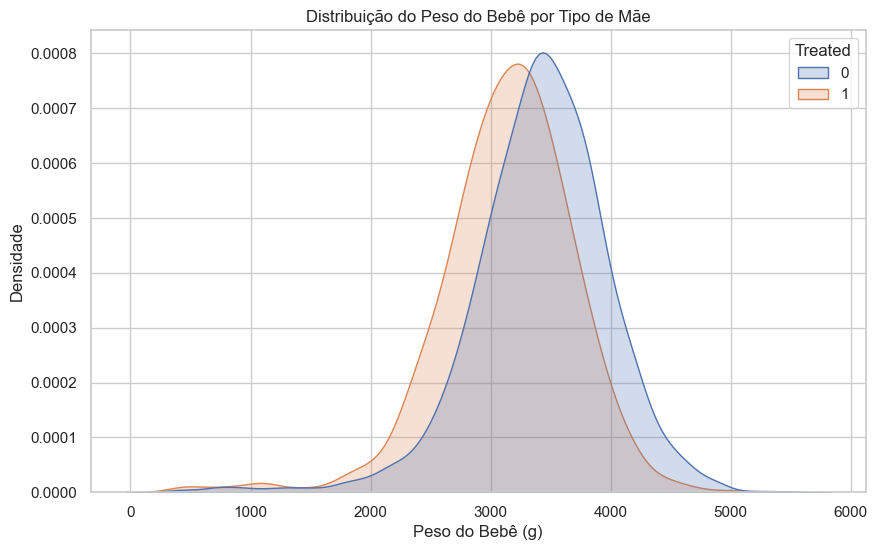
\includegraphics[width=0.5\textwidth]{Fig.png}
      \caption{\label{fig:Distribution} Distribuição do peso dos bebês.}
      \end{figure}
\section{Method}

Nós podemos representar a relação a ser estudada da seguinte forma:

\begin{equation}
Y = \alpha + \beta T + \gamma X + \epsilon
\end{equation}

\begin{equation}
T = \alpha + \beta Z + \gamma X + \epsilon
\end{equation}

Onde $Y$ é a variável dependente, $T$ é a variável tratamento, $X$ é o vetor de variáveis de controle, $\alpha$ é o intercepto, $\beta$ é o efeito causal do tratamento, $\gamma$ é o vetor de coeficientes das variáveis de controle, e $\epsilon$ é o termo de erro.

Segundo e terceiro parágrafos: Levantar as hipóteses teóricas de identificação da estratégia de identificação causal. Relacionar as hipóteses de identificação causal com o problema específico, no sentido de argumentar em favor do possível procedimento que está sendo utilizado (lembre das possíveis fontes de viés comentadas em aula). É importante elencar claramente as hipóteses de identificação causal do modelo econométrico utilizado, e argumentar em favor da validade dessas hipóteses na análise do problema específico.


\section{Results}

Dicas para o Primeiro parágrafo: [Validação da Análise]; dependendo do método utilizado, é conveniente apresentar os primeiros passos que o conduziu aos resultados encontrados. Por exemplo, uma etapa comum é apresentar o balanço das covariáveis para o caso de métodos de pareamento, ou apresentar o primeiro estágio do método de variáveis instrumentais, ou outros aspectos que validem a sua análise.

Dica para o Segundo parágrafo: [Apresentar os resultados em termos de magnitude, significância e relação com os mecanismos econômicos da relação]; após comentar os aspectos de validação da análise, apresentar os resultados numa outra tabela, e comentar seus efeitos, relacionando com os mecanismos (hipóteses levantadas na revisão da literatura)

\begin{table}[h]
\centering
      \caption{Results}
      \begin{tabular}{lrrr}
            \toprule
             & Treated-Model1 & Treated-Model2 & Treated-Model3 \\
             \midrule
             Effect & -275.2519 & -218.1870 & -203.0297 \\
             s.d. & 21.4528 & 22.0917 & 22.0547 \\
             T-test & -12.8306 & -9.8764 & -9.2057 \\
             P-value & 0.0000 & 0.0000 & 0.0000 \\
             N & 4642.0000 & 4642.0000 & 4642.0000 \\
             Adj. R-squared & 0.0341 & 0.0544 & 0.0870 \\
             \bottomrule
      \end{tabular} \\
\textbf{Notes:} A table using LaTeX
\end{table}


\section{Robustness Analysis}


Dicas para o Primeiro parágrafo: Apresentar todos os métodos de robustez, ex. placebo no tratamento, outros métodos adicionais não trabalhados nos resultados. Outras Amostras não consideradas. Lembre-se de que a ideia dessa seção e colocar os resultados encontrados a prova, e verificar se eles são fortes...

[Cada parágrafo subsequente explica de forma direta o método de robustez empregado e já apresenta os resultados encontrados]

\section{Discussion and Cost and Benefit Analysis}

\subsection{Discussion}

Aqui os autores têm uma certa liberdade para discutir os resultados encontrados, e relacioná-los com a literatura. É importante tentar explicar os resultados encontrados, e relacioná-los com os mecanismos causais levantados na revisão da literatura. Também é importante tentar explicar porque os resultados encontrados são diferentes dos resultados encontrados na literatura. **Os autores podem especular** sobre as razões para os resultados encontrados, e tentar relacioná-los com a realidade econômica. Ou seja, há uma certa liberdade para propor explicações para os resultados encontrados segundo a visão dos autores.

\subsection{Cost and Benefit Analysis}

Aqui os autores podem propor um exercício de política pública ou privada. A partir dos resultados econométricos (identificação causal), é possível calcular os impactos de possíveis políticas, e fazer análises de custo benefício.


\begin{table}[h]
      \centering
      \caption{Results}
      \begin{tabular}{cccccc}
          \toprule
          & Costs (R\$) & Interest (10\%) & Production & Inputs & Revenue \\
          \midrule
          Policy A & 20 million & 2 million & 5 MW & 576,000 & 3,360,000 \\
          Policy B & 200 million & 20 million & 50 MW & 5,760,000 & 33,600,000 \\
          Policy C & 400 million & 40 million & 100 MW & 11,520,000 & 67,200,000 \\
          Policy D & 2 billion & 200 million & 500 MW & 57,600,000 & 336,000,000 \\
          \bottomrule
      \end{tabular} \\
      \textbf{Notes:} A table using LaTeX
\end{table}

Dicas para o Terceiro Parágrafo: Apresentar as limitações da pesquisa, e propor sugestões para novas análises em caso de aprimoramento dos dados e/ou dos métodos a medida que a literatura avance.

\section{Final Remarks}

A seção de "Final Remarks" (Considerações Finais) de um artigo científico geralmente é reservada para sintetizar os principais pontos discutidos no estudo, destacar a importância dos resultados e propor possíveis direções para pesquisas futuras. 

O primeiro paragráfo deve reiterar os resultados principais (Comece reafirmando brevemente os resultados-chave alcançados em seu estudo. Isso ajuda a relembrar o leitor sobre a contribuição específica do seu trabalho para a área de estudo). E ressaltar as **Implicações e relevância** (Em seguida, discuta as implicações mais amplas dos seus resultados e por que eles são importantes para o campo. Isso pode incluir como seus achados se relacionam com teorias existentes, abrem novas áreas de investigação ou têm aplicações práticas.)

O Segundo parágrafo deve apresentar as **Limitações e considerações futuras** (reconheça qualquer limitação do seu estudo e sugira possíveis áreas para pesquisa futura. Isso mostra uma compreensão crítica do seu trabalho e abre espaço para outros pesquisadores expandirem sobre ele.)

O terceiro parágrafo deve Concluir (Conclua a seção de forma sucinta, reforçando a relevância do seu estudo e ressaltando sua contribuição para o conhecimento existente na área. Isso pode ser feito reafirmando a importância dos resultados ou destacando a inovação metodológica, e a aplicação dos achados em termos de políticas públicas ou privadas, por exemplo.)

Geralmente, essa seção pode ser escrita em dois a três parágrafos, dependendo da complexidade do estudo e da quantidade de pontos que precisam ser abordados. Lembre-se de manter a escrita concisa e direta ao ponto.

\newpage

\bibliographystyle{apalike}
\bibliography{Refs}

\end{document}